\documentclass[11pt,a4paper]{article}
\usepackage[utf8]{inputenc}\usepackage[T1]{fontenc}
\usepackage[margin=0.9in]{geometry}
\usepackage{amsmath,amssymb,booktabs,graphicx,enumitem,xcolor,parskip,titlesec}
\usepackage[hidelinks]{hyperref}
\graphicspath{{figures/}}
\definecolor{qnavy}{RGB}{20,40,75}\definecolor{qgrey}{RGB}{90,90,90}\definecolor{qred}{RGB}{150,30,30}
\definecolor{qgreen}{RGB}{47,107,79}
\titleformat{\section}{\large\bfseries\color{qnavy}}{\thesection}{0.6em}{}
\begin{document}\thispagestyle{empty}
\noindent
{\large\bfseries\color{qnavy} Report R23 --- Methylation and Drug Resistance in 187 Lung Cell
Lines}\\[2pt]
{\color{qgrey}A pre-registered test of the ``reprogramming resistance through epigenetic
modulation'' thesis. The verdict was CONTRADICTED. Its own post-hoc control then reversed the
sign, and neither reading is defensible.}\\[6pt]
{\color{qgrey}\rule{\textwidth}{0.4pt}}

\medskip
\noindent 20 August 2026 \quad\textbullet\quad Quantara \quad\textbullet\quad
{\color{qgrey}Peer-review audit copy}

\section*{Summary}

This replaces a set of figures that were entirely synthetic (see
\texttt{results/SIDEQUEST-lung-epigenetic-figures/}) with measurements on real data. The question
is the one that manuscript asserts: can epigenetic drugs be used against tumours that have become
resistant to standard therapy?

\textbf{Substrate.} 198 lung cell lines from GSE68379, processed from raw 450k IDATs
(485{,}512 probes), joined by COSMIC identifier to GDSC2 dose--response. \textbf{187 lines}
carry both. Histology: 64 lung adenocarcinoma, 58 small cell, 21 mesothelioma, 14 squamous,
13 large cell, 11 NSCLC not otherwise specified, 4 carcinoid, 2 other.

The analysis plan --- hypotheses, exclusions, gates, verdict thresholds and refusals --- was written
and SHA-256 hashed at \texttt{7e0322ba804aef2f\ldots} \emph{before any IC$_{50}$ was joined to any
methylation value}. The beta matrix was still being computed when the plan was hashed.

\subsection*{Three results}

\textbf{1. Methylation predicts drug sensitivity, and it is not subtle.} Ten of eleven
standard-of-care agents are predictable out-of-fold after Holm correction, and 14 of 32
chromatin-targeting drugs. Vorinostat reaches $\rho = 0.731$, Navitoclax $0.607$, Olaparib $0.536$,
Docetaxel $0.487$. Every EGFR inhibitor in the panel is predictable, Osimertinib included.

\textbf{2. The pre-registered primary test says the thesis is wrong.} Lines resistant to
standard-of-care are \emph{also} resistant to chromatin drugs: $\rho = +0.651$, permutation
$p = 0.0005$, $n = 187$. The plan's rule maps $\rho \geq +0.20$ with $p<0.05$ to
\textbf{THESIS\_CONTRADICTED}.

\textbf{3. That verdict does not survive its own control.} Both indices are mean $z$-scored
ln\,IC$_{50}$, so both load on a general drug-sensitivity axis --- some lines are simply resistant
to nearly everything. Partialling out an index built from \textbf{227 GDSC2 drugs in neither set}
takes the association from $+0.651$ to \textbf{$-0.160$} ($p = 0.033$). The sign \emph{reverses},
into the direction the thesis predicts, and lands below the pre-declared $-0.20$ threshold.

\textbf{So the honest answer is that this design cannot settle the question.} The pre-registered
test measured a confound. The corrected estimate is weakly in the thesis's favour and too small to
claim. Reporting either number alone would be misleading, and the plan did not anticipate the
confound.

\begin{center}
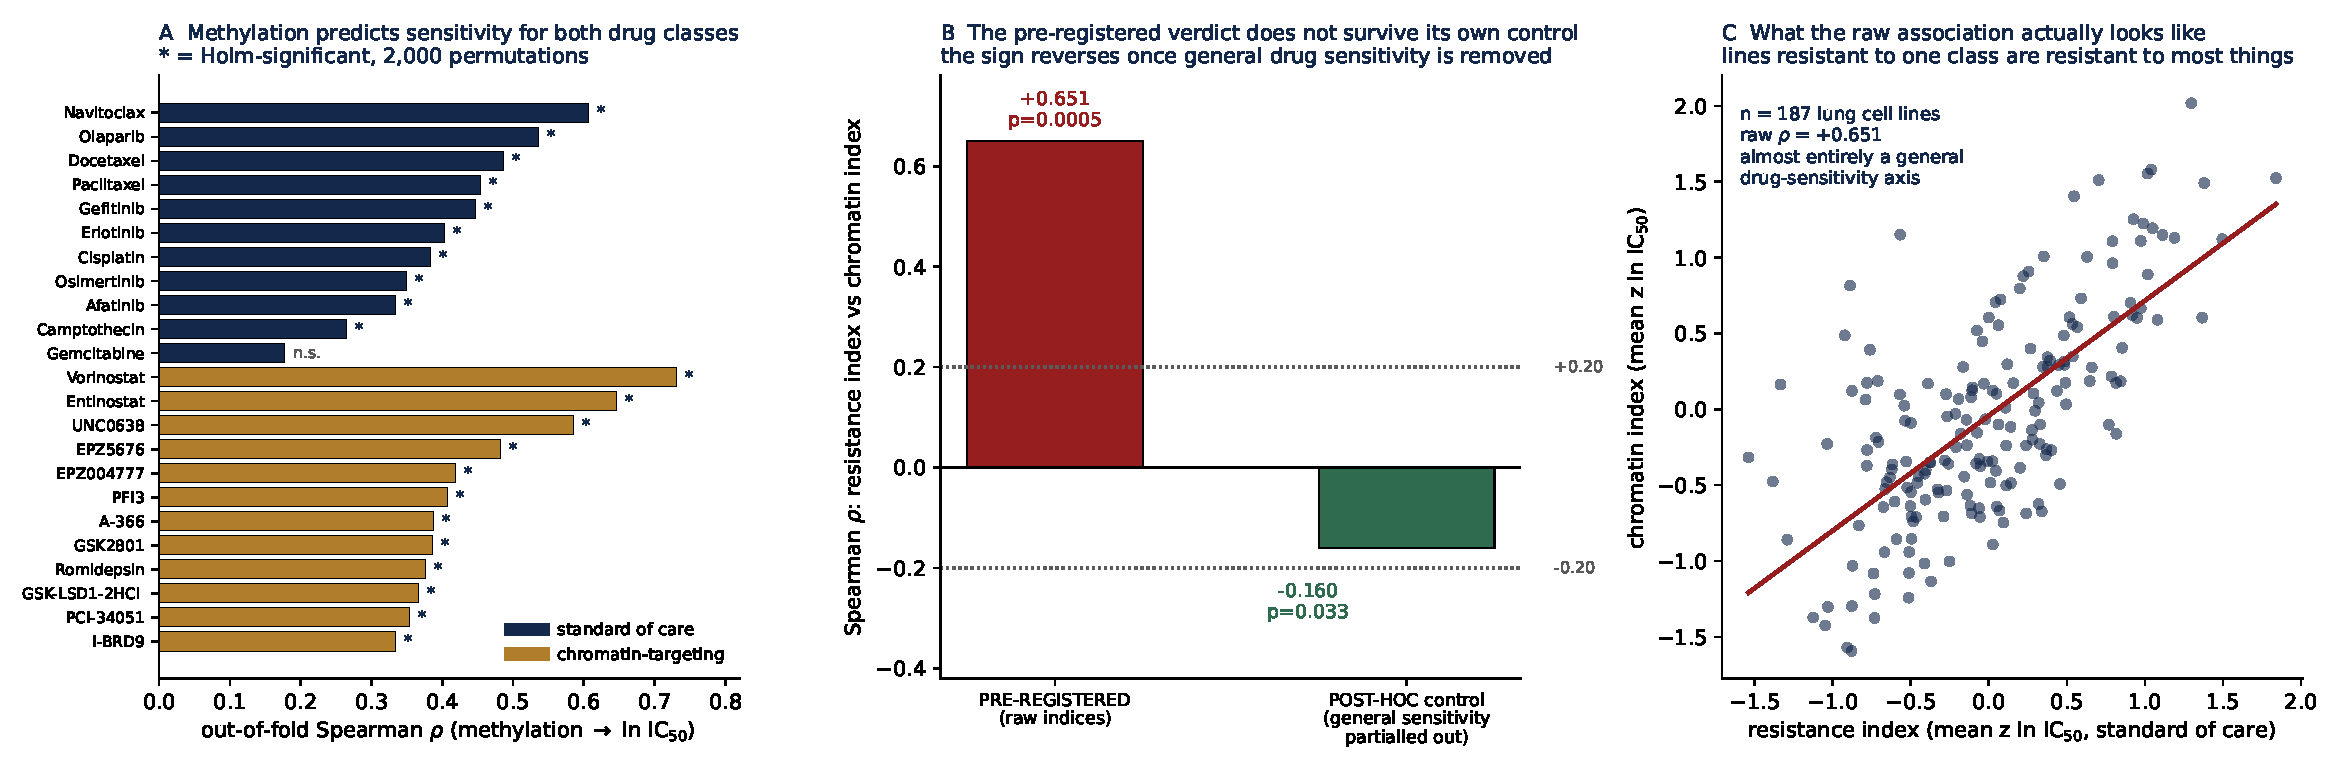
\includegraphics[width=\textwidth]{r23_panels.pdf}
\end{center}
\noindent{\small\color{qgrey}\textbf{A} Per-drug predictability, Holm-corrected over 2{,}000
permutations. \textbf{B} The primary test before and after the general-sensitivity control.
\textbf{C} The raw association, which is what a general sensitivity axis looks like.}

\section{Standard-of-care agents}

\begin{center}
\small
\begin{tabular}{@{}lrrr@{}}
\toprule
\textbf{Drug} & \textbf{$\rho$} & \textbf{$n$} & \textbf{Holm $p$} \\
\midrule
Navitoclax & 0.607 & 187 & 0.0055 \\
Olaparib & 0.536 & 187 & 0.0055 \\
Docetaxel & 0.487 & 187 & 0.0055 \\
Paclitaxel & 0.454 & 185 & 0.0055 \\
Gefitinib & 0.448 & 185 & 0.0055 \\
Erlotinib & 0.403 & 185 & 0.0055 \\
Cisplatin & 0.383 & 139 & 0.0055 \\
Osimertinib & 0.349 & 185 & 0.0055 \\
Afatinib & 0.334 & 187 & 0.0055 \\
Camptothecin & 0.265 & 187 & 0.0170 \\
Gemcitabine & 0.177 & 184 & 0.0555 \emph{(n.s.)} \\
\bottomrule
\end{tabular}
\end{center}

Top chromatin drugs: Vorinostat 0.731, Entinostat 0.646, UNC0638 0.586, EPZ5676 0.482,
EPZ004777 0.419 --- HDAC and histone-methyltransferase inhibitors respectively.

\textbf{A caveat that applies to this whole table.} These models may be predicting how sensitive a
line is \emph{in general} rather than its response to the specific drug. The same confound that
destroyed the primary test is not controlled here, and the plan did not require it to be. The
per-drug numbers should be read as ``methylation carries information about this line's IC$_{50}$'',
not as ``methylation predicts response to this agent specifically''.

\section{Two departures from the hashed plan}

Both logged rather than silently applied.

\textbf{The plan's permutation count made significance unreachable.} It specified 200
permutations, giving a $p$-floor of $1/201 = 0.00498$. Holm across 11 standard-of-care drugs cannot
then go below $0.0547$, and across 32 chromatin drugs cannot go below $0.159$. The first execution
duly reported \emph{zero} predictable drugs while Vorinostat sat at $\rho = 0.73$ --- an arithmetic
artefact of the plan, not a property of the data. Raised to 2{,}000 permutations, which can only
make rejection easier and never harder, and gate G6 now fails loudly if the floor is ever too
coarse for the family size again.

\textbf{Sex-chromosome probes could not be excluded.} Exclusion E5 required dropping them; the 450k
manifest is not staged locally, so no probe was dropped on that criterion. 385{,}096 probes were
retained after the missingness filter.

\section{Controls}

\begin{center}
\begin{tabular}{@{}llr@{}}
\toprule
\textbf{Gate} & \textbf{Check} & \textbf{Result} \\
\midrule
G0 & plan digest matches the pre-registration & PASS \\
G1 & 187 lines with both methylation and GDSC2 & PASS \\
G2 & 385{,}096 probes after filtering & PASS \\
PC1 & small-cell vs non-small-cell separable, balanced accuracy 0.892 & PASS \\
G3 & all permutation nulls within 0.05 of zero (max 0.021) & PASS \\
G4 & no drug retained below 100 lines (min 131) & PASS \\
G5 & resistance and chromatin indices use disjoint drug sets & PASS \\
G6 & permutation floor permits Holm significance & PASS \\
\bottomrule
\end{tabular}
\end{center}

PC1 matters: it establishes the beta matrix carries real biology before any drug association is
interpreted. Small-cell and non-small-cell lung lines separate at 0.892 balanced accuracy from
methylation alone.

\section{A data-integrity finding}

Our mirror of \texttt{GSE68379\_RAW.tar} is \textbf{corrupt and fails silently}. It is
byte-complete against both GCS and GEO's declared size (9{,}020{,}579{,}840), ends with a valid tar
terminator, and raises no error --- but enumerates \textbf{1{,}302 of 2{,}056 members}, 649 of
1{,}028 cell lines, 127 of 198 lung. Two extraction modes gave the identical truncation.

It was caught only because the job asserted an expected array count and halted. The 396 lung IDATs
were then fetched per sample from GEO instead: 396 of 396, zero failures. The data inventory
describes this archive as 1{,}028 cell lines, which is true of GEO's copy and not of ours.

\section{Limitations}

\textbf{Cell lines are not tumours.} Methylation drifts in culture and ln\,IC$_{50}$ is a
laboratory phenotype. Nothing here speaks to a patient, and the plan's refusals forbid saying
otherwise.

\textbf{The primary question is unresolved, not answered.} A corrected pre-registration would
build both indices on residuals after removing the general-sensitivity axis, and would declare that
before looking.

\textbf{187 lines against 485{,}512 probes.} Every model is heavily regularised and only the
out-of-fold estimate is reported.

\textbf{Mixed histology.} 58 of 187 are small cell and 21 mesothelioma, which differ from NSCLC in
both methylation and drug response. No histology-stratified analysis was pre-declared.

\textbf{Hash-before-label only.} The plan author and the executor are the same person, so this is
the weaker form of the protocol, not the structurally isolated form used in R16.

\section*{Reproducing this report}

\texttt{evidence/PREREG\_PLAN.yaml} (hashed \texttt{7e0322ba804aef2f\ldots}),
\texttt{evidence/PREREGISTRATION.json}, \texttt{evidence/run\_analysis.py},
\texttt{evidence/process\_idats.py} (GEO fetch and methylprep),
\texttt{evidence/diagnose\_tar.py} (the archive diagnostic),
\texttt{evidence/results.json}, \texttt{evidence/gates.json},
\texttt{evidence/resistance\_index.npy}, \texttt{evidence/chromatin\_index.npy}.
Figure: \texttt{python3 make\_figure.py}.

\end{document}
